\chapter{Perancangan}
\label{chap: Perancangan}

Pada bab ini akan dibahas mengenai perancangan perangkat lunak yang diimplementasi pada pohon kurikulum.

\section{Kebutuhan \textit{Input} dan \textit{Output}}
\label{sec: Kebutuhan Input dan Output}
Perancangan perangkat lunak pohon kurikulum dengan men \textit{generate} dari JSON ke \textit{DOT}. Input perangkat lunak merupakan kode, nama, prasyarat, sks, semester, dan wajib.
Kebutuhan input dan output perangkat lunak:
\begin{itemize}
\item \textit{Input} \\
Kebutuhan \textit{input} pada pohon kurikulum adalah
\begin{enumerate}
\item \textbf{kode}, berisikan kode mata kuliah
\item \textbf{nama}, berisikan nama mata kuliah
\item \textbf{sks}, memberitahukan kepada mahasiswa mata kuliah yang akan diambil memiliki beban berapa banyak.
\end{enumerate}
\item \textit{Output}\\
Output dari perangkat lunak adalah pohon kurikulum.
\end{itemize}

\section{Memanggil \textit{Library} dan Membuat \textit{Server}}
\label{sec: Memanggil Library dan Membuat Server}

Pada gambar \ref{fig: lib dan server} terdapat dua bagian yang bisa dijelaskan yaitu:
\begin{enumerate}
\item Baris 1-3 berfungsi untuk memanggil \textit{library} yang akan digunakan.
\item Baris 5-16 membuat server yang akan dijalankan di dalam \textit{node.js}. Di dalam createServer ini terdapat variabel \textit{graphDot} yang menampung \textit{ranksep, nodesMatkul} ,dan \textit{edgesMatkul}.
\end{enumerate}

\begin{figure}[H]
		\centering
		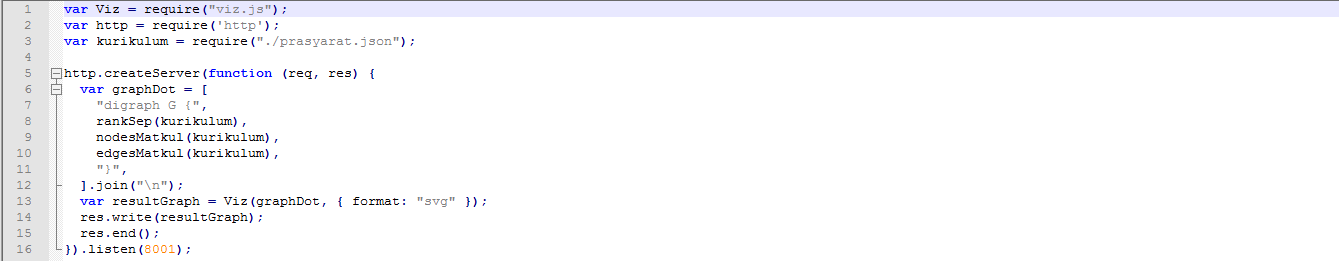
\includegraphics[scale = 0.6]{libdanserver.png}
		\caption{Library dan Create Server}
		\label{fig: lib dan server}
\end{figure}	

\section{Membuat rankSep}
\label{sec: Membuat rankSep}
\textit{RankSep} adalah pemisah antara posisi atas dan posisi bawah. \textit{RankSep} biasanya diukur dalam inci. Di gambar \ref{fig: ranksep} terdapat fungsi \textit{rankSep}. Fungsi ini akan menampilkan kode-kode mata kuliah wajib yang ada di tiap semester. 

\begin{figure}[H]
		\centering
		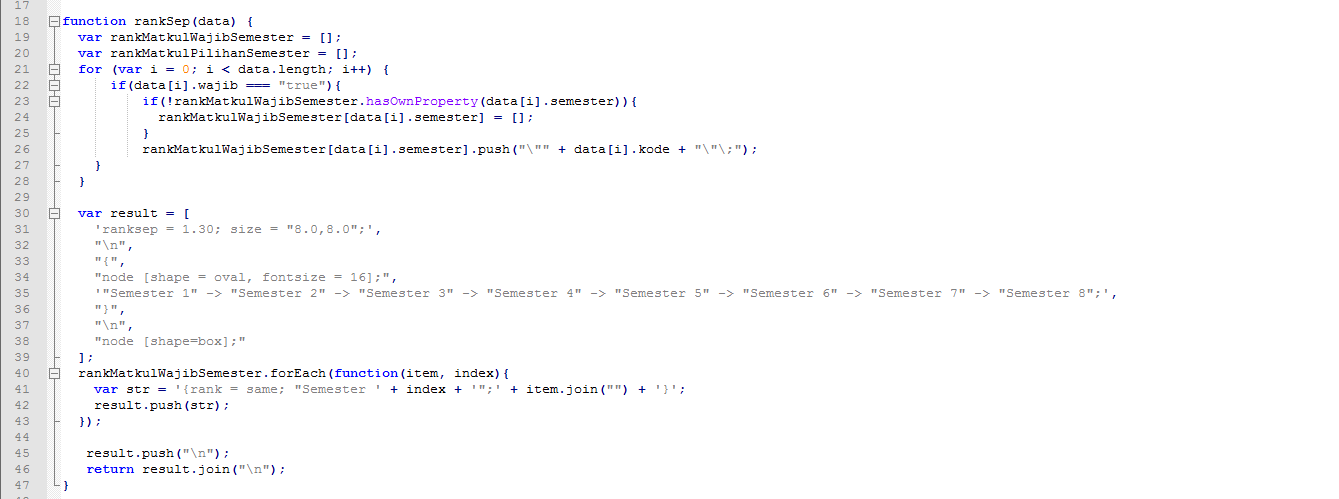
\includegraphics[scale = 0.6]{ranksep.png}
		\caption{ranksep}
		\label{fig: ranksep}
\end{figure}	

\section{Membuat \textit{nodesMatkul}}
\label{sec: Membuat nodesMatkul}
\textit{NodesMatkul} berisikan kode matakuliah, sks, dan nama mata kuliah yang ada di tiap semester. \ref{fig: nodeMatkul}. \textit{Node} hanya akan berisikan mata kuliah wajib.

\begin{figure}[H]
		\centering
		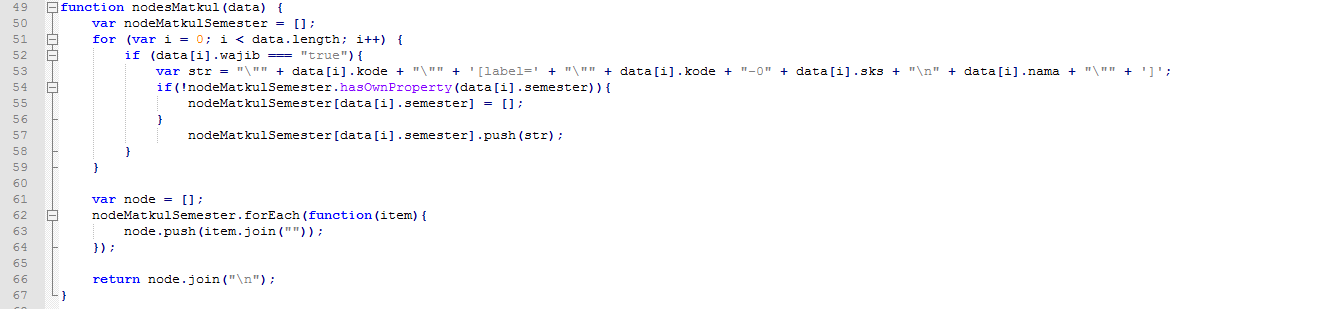
\includegraphics[scale = 0.6]{node.png}
		\caption{node mata kuliah}
		\label{fig: nodeMatkul}
\end{figure}	

\section{Membuat \textit{edgesMatkul}}
\label{sec: Membuat edgesMatkul}
\textit{EdgesMatkul} memiliki fungsi untuk menunjukkan apakah mata kuliah yang akan di ambil memiliki syarat atau tidak. Syarat dapat berupa syarat tempuh, syarat lulus, atau bersamaan. Pada gambar \ref{fig: edgeMatkul}. Dapat dilihat jika mata kuliah tersebut memiliki syarat lulus maka hasilnya garis akan lurus memanjang sedangkan jika mata kuliah tersebut memiliki syarat tempuh maka garis akan membentuk putus-putus mengarah pada mata kuliah yang memiliki syarat tempuh tersebut.

\begin{figure}[H]
		\centering
		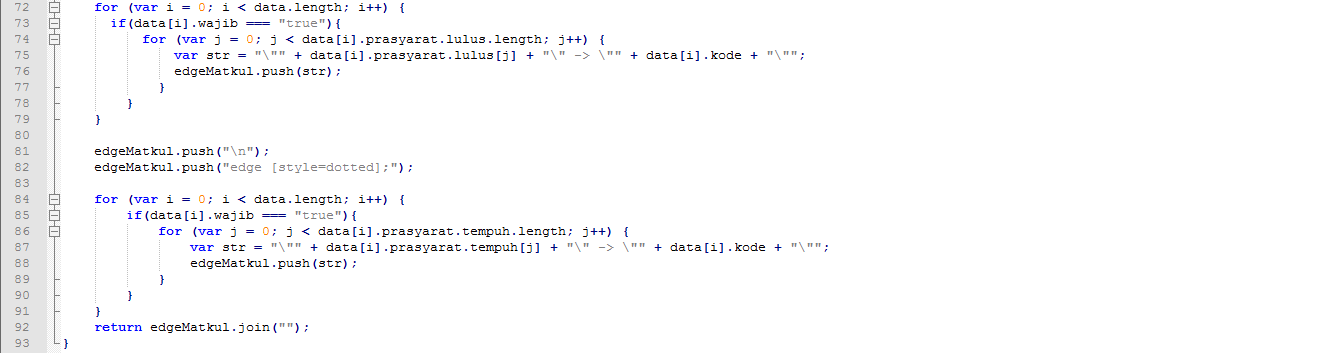
\includegraphics[scale = 0.6]{edge.png}
		\caption{edge mata kuliah}
		\label{fig: edgeMatkul}
\end{figure}	
